\section{Declared extension: observable geometry and corrected tail betting}
\label{sec:tail-extension}
This section develops an exploratory extension after the baseline pilot.
The baseline and its inactive portfolios remain reported unchanged. The
extension uses stronger moment information, and its first-entry experiment
does not establish the performance of a complete adaptive strategy.
Linear betting factors and their mixtures belong to the existing testing-by-
betting literature \cite{boundedbet}; the contribution here is an explicit
policy-moment envelope and a bias-corrected specialization, not a claim to
have invented linear betting or mixtures.

\subsection{A public envelope without hidden signal labels}
Let $Z_t^{fun}$ be the $N\times p$ matrix of observable function values and
$P_t$ the observable sleeve holdings before the next stock return $R$.
For a stock allocation $q=P_tw$, conditional return mean is
$q'Z_t^{fun}\theta_t$. Replace knowledge of the true support by the public
relaxation
\[
 \Theta=\{\theta\in\mathbb R^p:0\le\theta_j\le u,
                          \ \textstyle\sum_j\theta_j\le T\}.
\]
Here $u$ is the largest coefficient cap and $T$ the sum of group caps; every
signal identifier receives the same cap. Knowing these two aggregate bounds
does not identify which 55 coefficients are zero.

For a vector $a$, the support function $h_\Theta(a)$ fills the largest
positive coordinates of $a$ at rate $u$ until budget $T$ is exhausted,
including a fractional final coordinate. Thus
\[
 m(q)=\max\{h_\Theta((Z_t^{fun})'q),
             h_\Theta(-(Z_t^{fun})'q)\}
\]
bounds the absolute conditional mean. This is a deterministic linear-program
bound, not a fitted mean or an oracle coefficient.

Suppose factor loadings satisfy public componentwise intervals
$\beta_{ik}\in[c_k-r_k,c_k+r_k]$, factor scales are at most $\bar\sigma_k$
and idiosyncratic scales at most $\bar\sigma_e$. Independence of the
standardized Laplace shocks gives the variance bound
\begin{equation}
 v(q)=\sum_k\bar\sigma_k^2
       (|c_k\mathbf 1'q|+r_k\norm q_1)^2
       +\bar\sigma_e^2\norm q_2^2.\label{eq:public-geometry}
\end{equation}
The last term retains cross-sectional diversification rather than replacing
the stock $L_2$ norm by gross leverage. The generator implies intervals
$[.5,1.5]$ for the first beta and $[-1,1]$ for the other three. The
individual realized beta vector remains hidden. Risk scales cover the larger
of the normal and stress levels. Dollar neutrality cancels the common center
of the first loading interval.

For $x=\mu+h'\zeta$ and independent standardized Laplace shocks, put
$\norm h_2^2\le v$, $|\mu|\le m$. For even $\ell\le8$ define
\begin{equation}
 H_\ell(m,v)=\sum_{k=0}^{\ell/2}
  \binom{\ell}{2k}m^{\ell-2k}(2k)!(v/2)^k.\label{eq:laplace-upper-even}
\end{equation}
Then $\E x^\ell\le H_\ell(m,v)$. To see this, the even Taylor coefficient of
$\prod_j(1-h_j^2z^2/2)^{-1}$ is bounded by the corresponding coefficient
of $(1-vz^2/2)^{-1}$: each monomial in the former occurs with a multinomial
coefficient at least one in the latter. Hence
$\E(h'\zeta)^{2k}\le(2k)!(v/2)^k$; binomial expansion supplies
\eqref{eq:laplace-upper-even}. No moment-generating assumption is imposed
directly on the quadratic utility score.

For two policies, write $d=q_B-q_S$, $s=q_B+q_S$ and predictable
$D=C_B-C_S$. Their score is $Y=d'R-\gamma(d'R)(s'R)/2-D$.
Let $H_{\ell,d}=H_\ell(m(d),v(d))$ and similarly for $s$.
Minkowski and conditional Cauchy--Schwarz give
\begin{align}
 V_2&=\left\{H_{2,d}^{1/2}
       +\frac\gamma2(H_{4,d}H_{4,s})^{1/4}+|D|\right\}^2,
       \label{eq:geometry-second}\\
 V_4&=\left\{H_{4,d}^{1/4}
       +\frac\gamma2(H_{8,d}H_{8,s})^{1/8}+|D|\right\}^4,
       \label{eq:geometry-fourth}
\end{align}
as conditional bounds on $\E Y^2$ and $\E Y^4$. For example,
$\norm{(d'R)(s'R)}_{L_4}\le
(\E(d'R)^8\E(s'R)^8)^{1/8}$. These computations may be verified
conditional on the simulator's larger filtration; because the bounds use only
public pre-return quantities, the tower property gives the same envelopes
for the learner's filtration. If targets coincide but prior states differ,
$d=0$ and these formulas give exactly $D^2,D^4$.

\subsection{Bias-corrected lower winsorization}
For $p>1$, $B>0$ and $x\ge0$,
\begin{equation}
 (x-B)_+\le\frac{(p-1)^{p-1}}{p^p}\frac{x^p}{B^{p-1}}.\label{eq:sharp-tail}
\end{equation}
The maximum of $(x-B)/x^p$ for $x\ge B$ is attained at
$x=pB/(p-1)$, which proves both the inequality and its sharp constant.
For predictable envelopes $V_{2,t},V_{4,t}$ define
\begin{equation}
 b_t=\min\left\{\frac{V_{2,t}}{4B_t},
                       \frac{27V_{4,t}}{256B_t^3}\right\},\qquad
 X_t=\max\{Y_t,-B_t\}-b_t.\label{eq:corrected-score}
\end{equation}
Only the downside is winsorized; upside may remain unbounded.

\begin{theorem}[A corrected-tail e-process for the original utility null]
Suppose $B_t>0$ is predictable and the two moment envelopes are valid. Under
$\E[Y_t\mid\F_{t-1}]\le0$, the factors
\[
 Q_t=1+\lambda_t X_t,\qquad
 0\le\lambda_t\le\rho/(B_t+b_t),\quad 0<\rho<1,
\]
have conditional expectation at most one and satisfy $Q_t\ge1-\rho>0$.
Their product is a nonnegative test supermartingale for the original null.
Any fixed convex mixture of these products has the same guarantee.
\end{theorem}
\begin{proof}
The increase caused by winsorization is $(-B_t-Y_t)_+$. Apply
\eqref{eq:sharp-tail} to $(-Y_t)_+$, using either moment bound, to obtain
\[
 \E[(-B_t-Y_t)_+\mid\F_{t-1}]\le b_t.
\]
Consequently $\E[X_t\mid\F_{t-1}]\le\E[Y_t\mid\F_{t-1}]\le0$.
Since $X_t\ge-B_t-b_t$, the stated bound on $\lambda_t$ guarantees
positivity. Predictability gives $\E[Q_t\mid\F_{t-1}]\le1$; multiplication
and linearity prove the product and mixture statements.
\end{proof}

Clipping without subtracting the bias can reverse the null mean. For
example, a mean-zero distribution with a rare large negative observation
becomes positively biased after lower clipping. The correction is therefore
part of the test, not an optional robustness adjustment. The fourth-moment
route requires eighth return moments, a stronger assumption than baseline
T1. A sample fourth moment alone does not supply this certificate.

\subsection{A power certificate and the mixture price}
Suppose under an alternative that $\E[Y_t\mid\F_{t-1}]\ge\delta_t$.
Because winsorization increases the score,
$\E X_t\ge\delta_t-b_t$ conditionally. Also
$\E[X_t^2\mid\F_{t-1}]\le(\sqrt{V_{2,t}}+b_t)^2=:W_t$.
For $z\ge-\rho$,
\[
 \log(1+z)\ge z-\frac{z^2}{2(1-\rho)},\qquad
 \frac1{1+z}\le1-z+\frac{z^2}{1-\rho}.
\]
The second inequality follows from
$(1+z)^{-1}=1-z+z^2/(1+z)$; the first follows by differentiation.
Thus conditional expected log growth is at least
\[
 \lambda_t(\delta_t-b_t)-\frac{\lambda_t^2W_t}{2(1-\rho)}.
\]
For a fixed mixture component, put
$g_t=\lambda_t(\delta_t-b_t)-\lambda_t^2W_t/(1-\rho)$.
The inverse-capital process compensated by $\exp(\sum g_t)$ is a
nonnegative supermartingale. If $\sum_{t\le hK}g_t\ge G_K$ almost surely,
the same endpoint Markov argument as T2a gives the mixture power bound
\begin{equation}
 \Prb\left(\max_{k\le K}E^{mix}_{hk}\ge1/\alpha\right)
 \ge\left[1-\frac{e^{-G_K}}{\alpha\omega}\right]_+,
\end{equation}
where $\omega$ is that component's fixed mixture weight. This is a lower
certificate under explicit alternative assumptions, not an exact power
optimum. Pathwise $\log E^{mix}_t\ge\log E^{component}_t+\log\omega$;
nine equally weighted components cost at most $\log9$ relative to one.

\subsection{A local information cost of moment-only certification}
Conservative moment information can impose a genuine cost even when an
alternative generates an entirely stable positive score. The following
two-point indistinguishability argument is local to that benign alternative;
it is not a minimax rate over all positive-mean distributions. Such rare-event
constructions are standard tools in heavy-tail inference; see the broader
discussion in \cite{heavysurvey}.

\begin{proposition}[A rare-loss lower bound]
Consider any possibly randomized sequential rule with probability at most
$\alpha$ of ever rejecting under every i.i.d. law having nonpositive mean,
second moment at most $v_2$ and fourth moment at most $v_4$. Let $P_\delta$
put mass one at $\delta>0$. For any $0<\varepsilon<1$ satisfying
\begin{equation}
 \delta^2\frac{1-\varepsilon}{\varepsilon}\le v_2,\qquad
 \delta^4\left\{1-\varepsilon+
              \frac{(1-\varepsilon)^4}{\varepsilon^3}\right\}\le v_4,
 \label{eq:rare-loss-moments}
\end{equation}
the probability of rejection by observation $n$ under $P_\delta$ is at most
$\min\{1,\alpha(1-\varepsilon)^{-n}\}$. A necessary condition for power
at least $1-\beta$ by $n$ is
\begin{equation}
 n\ge\frac{\log\{(1-\beta)/\alpha\}}
                  {-\log(1-\varepsilon)}.\label{eq:rare-loss-horizon}
\end{equation}
\end{proposition}
\begin{proof}
Take an i.i.d. null $Q$ with mass $1-\varepsilon$ at $\delta$ and mass
$\varepsilon$ at $-\delta(1-\varepsilon)/\varepsilon$. Its mean is zero
and its moments are exactly the two expressions in
\eqref{eq:rare-loss-moments}. With probability $(1-\varepsilon)^n$, its
first $n$ observations are all $\delta$. On that event the observed history
is identical to the history under $P_\delta$; the rule's independent
randomization has the same law. Thus, for rejection event $A_n$,
\[
 \alpha\ge Q(A_n)\ge(1-\varepsilon)^nP_\delta(A_n).
\]
Rearranging proves both statements.
\end{proof}

For example, if
$\varepsilon=\max\{\delta^2/v_2,(2\delta^4/v_4)^{1/3}\}\le1/2$,
both inequalities hold. Indeed the fourth moment is at most
$2\delta^4/\varepsilon^3$. With a second-moment restriction alone one may
use $\varepsilon=\delta^2/(v_2+\delta^2)$. For small $\delta$, these
constructions give local necessary horizons of orders
$v_2\delta^{-2}$ and $v_4^{1/3}\delta^{-4/3}$, respectively, up to
the logarithmic confidence factor. With both restrictions, the displayed
construction has order the smaller of these two expressions.

The corrected-tail construction attains the corresponding local order at
a predeclared design effect. For a single known $p$th-moment bound $M_p$,
put $\kappa_p=(p-1)^{p-1}/p^p$ and choose
\[
 B=(2\kappa_pM_p/\delta)^{1/(p-1)},\quad b=\delta/2,\quad
 \lambda=\rho/(B+b),\quad 0<\rho<1.
\]
This is a valid test by the clipping proof, and under the deterministic
alternative its capital is exactly
\[
 E_n=\left(1+\frac{\rho\delta}{2(B+\delta/2)}\right)^n.
\]
Consequently its crossing horizon is of order
$M_p^{1/(p-1)}\delta^{-p/(p-1)}\log(1/\alpha)$ as $\delta\to0$.
Here the design effect is fixed before testing; this calculation does not
license fitting it to the observations used to establish significance.
It is an order comparison at a deterministic alternative, not an optimality
claim for the nine-component implementation or the changing financial DGP.
The two-point null need not belong to the fixed Laplace market: the lower
bound applies to guarantees over a full moment class, and can be avoided by
legitimately exploiting stronger distributional information.

\begin{corollary}[An opportunity cost of certification in a single gate]
Consider the costless single-candidate subcase, with an incumbent of zero
utility and deterministic candidate utility $0<\delta\le1/(2\gamma)$ per period. A fund
remains with the incumbent until the first rejection time $\tau$, then
deploys the candidate in the next period. Under the assumptions of the
rare-loss proposition, its expected cumulative utility loss over $T$ periods
relative to immediate deployment is at least
\begin{equation}
 \delta\sum_{n=0}^{T-1}
       \left[1-\alpha(1-\varepsilon)^{-n}\right]_+.
 \label{eq:certification-opportunity-cost}
\end{equation}
\end{corollary}
\begin{proof}
Under the deterministic alternative, lost utility is exactly
$\delta\min(\tau,T)$. For an integer-valued stopping time,
$\E\min(\tau,T)=\sum_{n=0}^{T-1}\Prb(\tau>n)$.
The preceding proposition bounds each complementary crossing probability,
which proves \eqref{eq:certification-opportunity-cost}.
\end{proof}
This is a single-comparison result in a costless subcase; it neither provides
a regret bound for the uncorrected search over 100 signals nor treats the
additional trading-state costs of the financial experiment. It isolates a
mechanism: evidence waiting can have economic cost even before frictions are
introduced. It does not assert that the observed twelve-year waits are
necessary in the Laplace market.
An explicit quadratic-utility representation takes
$r_+=2\delta/(1+\sqrt{1-2\gamma\delta})$ and
$r_-=-2a/(1+\sqrt{1+2\gamma a})$, with
$a=\delta(1-\varepsilon)/\varepsilon$. Then $U(r_+)=\delta$ and $U(r_-)=-a$.
This embeds the score null in a fixed ENTRY comparison. It need not preserve
additional public return-moment restrictions and does not apply to cash-PARK
classes whose economic lower bound excludes the arbitrarily large negative score.

The proposed mechanism experiment fixes scales $c\in\{2,4,8\}$,
$B_t=cV_{4,t}^{1/4}$, and fractions $\rho\in\{.25,.5,.75\}$ before
using new seeds 40001--40020. It retains all nine components in the mixture.
Each candidate remains a single-sleeve shadow policy against the empty
reference, and all test arms use exactly the same realized scores. Only
annual first-entry feasibility is evaluated. Any observations from these new
markets are exploratory evidence for this declared extension; they neither
replace the old pilot nor constitute a full strategy or final-study result.

\IfFileExists{generated_tail_results.tex}{\subsection{Executed first-entry mechanism study}

The executed mechanism study contains 20 fresh markets from seeds 40001--40020, using $N=500$, $p=100$ and the 15-year DGP of the baseline. The four arms share every candidate shadow policy and every realized utility score. All 100 comparisons remain under observation to the common horizon, including after crossing. These are fixed-reference mechanism experiments, not twenty new full-strategy backtests.

\begin{table}[H]\centering\small

\begin{tabular}{lrrrr}

\toprule

Arm & Entry markets & Before end & Median year & Max. log E \\

\midrule

Catoni--baseline & 0/20 & 0/20 & NA & 0.008 \\

Catoni--geometry & 0/20 & 0/20 & NA & 0.555 \\

Tail--uniform & 0/20 & 0/20 & NA & 0.710 \\

Tail--geometry & 19/20 & 18/20 & 12.0 & 4.918 \\

\bottomrule\end{tabular}

\caption{Annual eligible first-entry events. ``Before end'' excludes a first crossing at the terminal revision. Median year is conditional on crossing; censored markets remain in the entry-rate denominator. No actual post-entry fund path is simulated.}\end{table}

The corrected-tail geometric arm has 19 entry markets out of 20; the Wilson 95\% interval for this market-level fraction is [0.764, 0.991]. It is a search outcome over 100 candidates, not an individual-test power estimate or a globally controlled rejection probability. One first certification occurs only at the terminal revision; 18 markets have any remaining market observations after certification. Neither geometric Catoni nor uniform-moment corrected-tail betting alone produces an entry in these 20 markets. The combined change improves statistical feasibility but does not remove the substantial cost of waiting.

4 selected first policies use structural proxies whose own coefficient is fixed at zero in the generator. Their conditional shadow gains are positive on the last evaluated date before selection. This illustrates the distinction between structural and economic relevance; it is not a false-discovery calibration result. These conditional gains refer to the shadow state, not a claim that the fund can acquire the shadow positions without paying its actual entry cost.

An additional post-hoc action audit replays all selected histories, refits with then-available observations and computes a hypothetical next-period entry from the fund's actual zero allocation. It values that action with true current model moments after selection, without drawing the next return. 18 of 18 nonterminal entries have positive conditional utility after actual entry costs. The mean is 0.957 basis points of daily utility, compared with 2.457 for the continuing shadow; the actual entry cost is 1.500 basis points. This conditional action valuation is descriptive and supplies no post-entry fund path or new guarantee of current profitability.

Separate predictable skew-null diagnostics use 10,000 independent paths and 2,000 observations. The corrected mixture crosses at rate 0.0068 (Wilson interval [0.0054, 0.0086]). An invalid single bettor ($B_t=V_{4,t}^{1/4}$, fraction $.75$) without bias correction crosses at rate 0.9966. This is an invalidity demonstration; its configuration differs from the mixture, so it is not a matched power comparison.

\begin{figure}[H]\centering

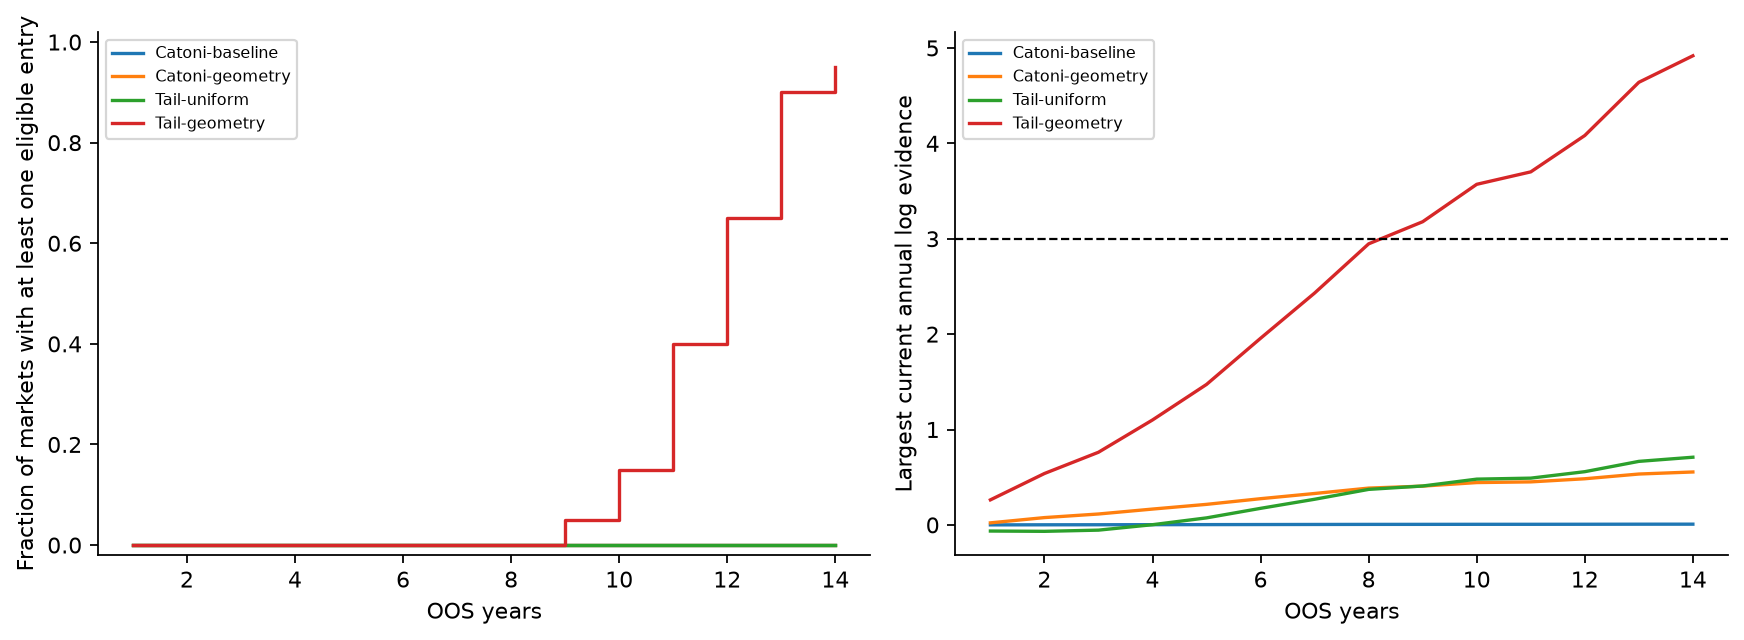
\includegraphics[width=.97\linewidth]{figures/first_entry_feasibility.png}

\caption{First-entry feasibility across twenty complete fresh markets. Every arm uses the same scores. Curves include terminal test events, with no claim of post-entry trading performance.}

\end{figure}

\begin{figure}[H]\centering

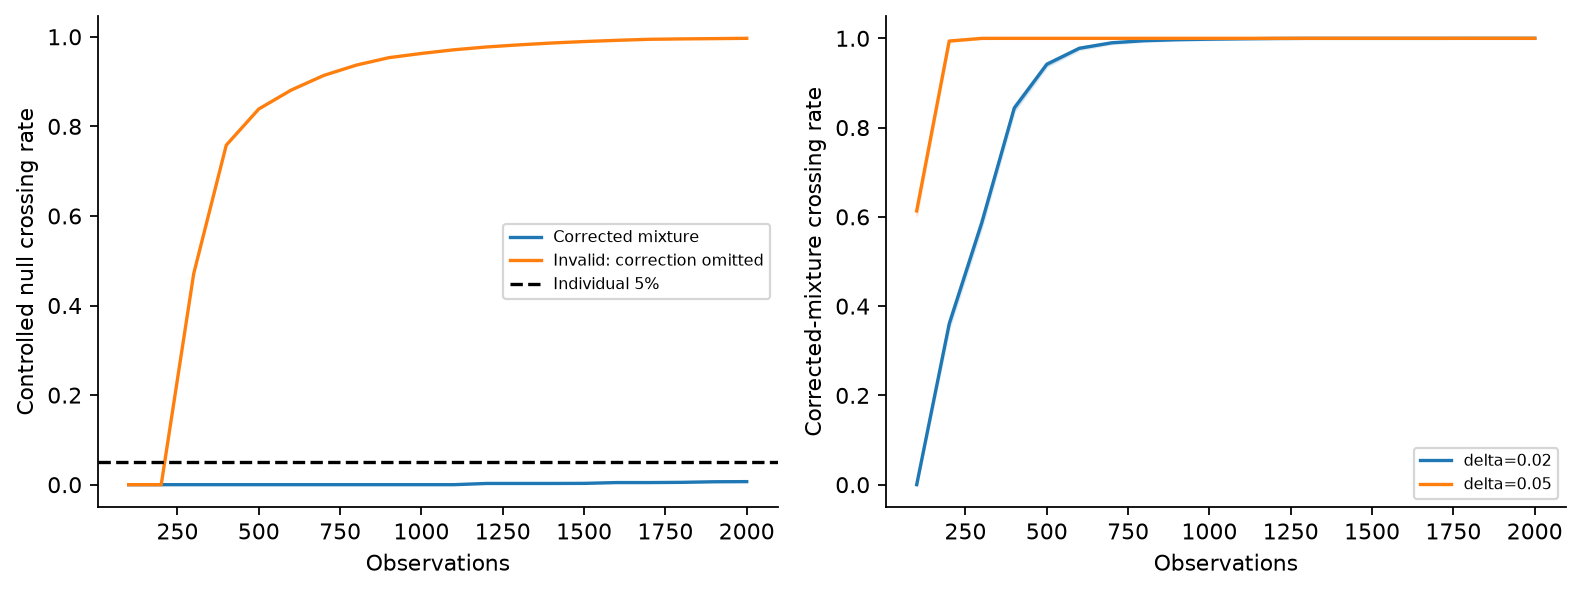
\includegraphics[width=.97\linewidth]{figures/controlled_tail_calibration.png}

\caption{Controlled statistical experiment under a predictable skewed null and two positive-mean alternatives. The invalid negative control is a single uncorrected bettor; it is not a matched power comparison with the corrected mixture. Shading shows Wilson intervals across independent paths.}

\end{figure}

\FloatBarrier
}{}
